\section{Обзор и классификация методов}

\begin{frame}{Два подхода к понижению размерности}
    \textbf{Отбор признаков:}
    \begin{itemize}
        \item Выбор подмножества исходных признаков.
        \item Сохранение информации без преобразования данных.
    \end{itemize}

    \textbf{Преобразование признаков:}
    \begin{itemize}
        \item Трансформация данных в новое пространство меньшей размерности.
        \item Сохраняет наиболее значимые свойства данных.
    \end{itemize}

    \begin{figure}
        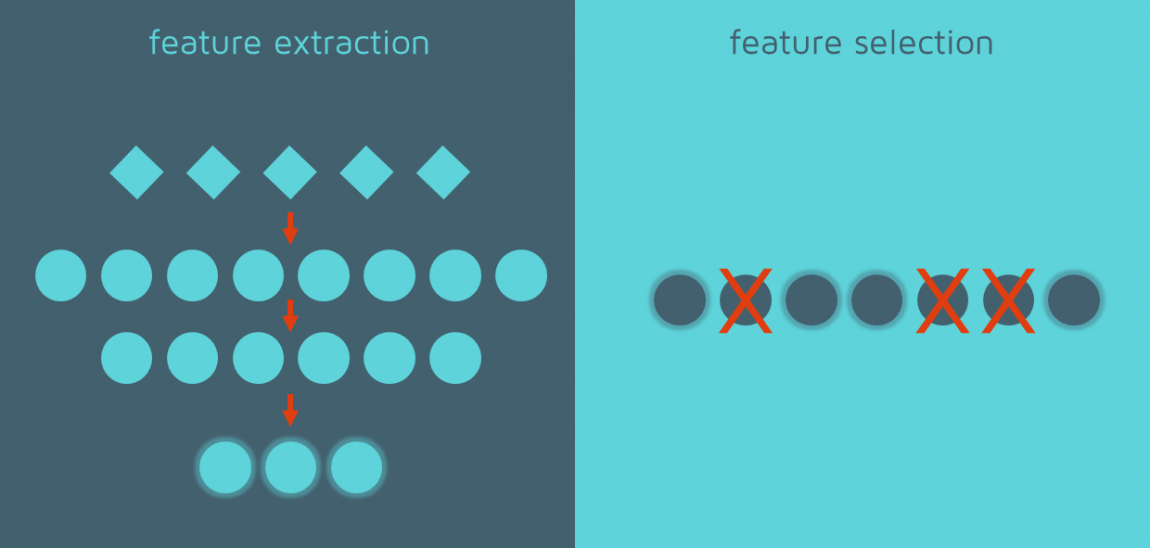
\includegraphics[width=.5\textwidth]{../resources/methods/feature_selection_vs_extraction.png}
    \end{figure}
\end{frame}

\subsection{Линейные методы}

\begin{frame}{Principal Component Analysis (PCA)}
    \textbf{Цель:} Сохранить максимальную дисперсию данных.

    \textbf{Пример применения:}
    \begin{itemize}
        \item Визуализация данных высокой размерности (например, геномика).
        \item Уменьшение размерности для кластеризации образцов.
    \end{itemize}

    \begin{figure}
        \centering
        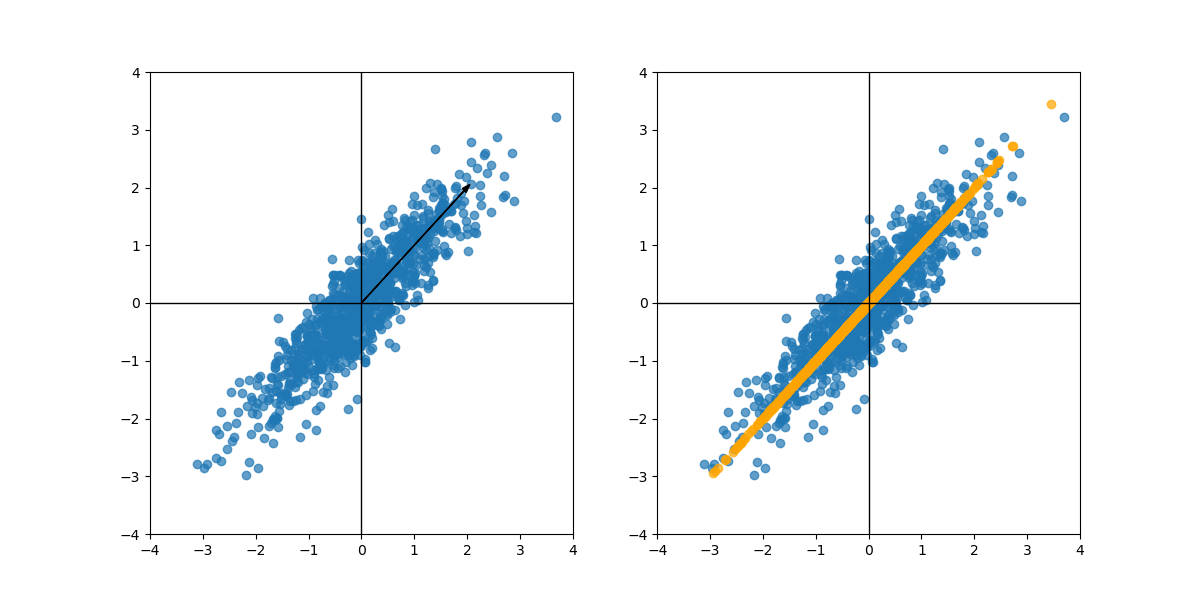
\includegraphics[width=.55\textwidth]{../resources/methods/pca.png}
    \end{figure}

\end{frame}

\begin{frame}{Sparse PCA (SPCA)}
    \textbf{Отличие от PCA:}
    \begin{itemize}
        \item Ограничение на разреженность главных компонент.
        \item Уменьшает сложность интерпретации данных.
    \end{itemize}

    \textbf{Применение:}
    \begin{itemize}
        \item Анализ данных с множеством нерелевантных признаков (например, финансовые индикаторы).
    \end{itemize}

    \begin{figure}
        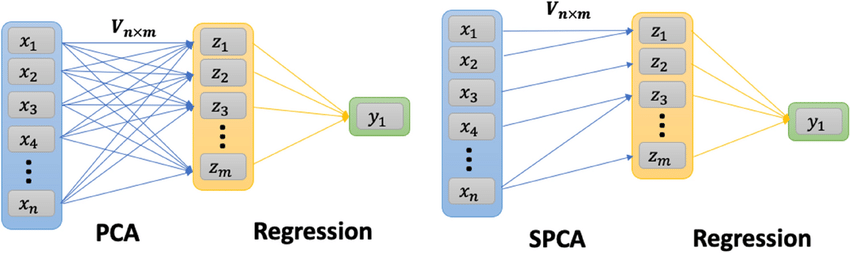
\includegraphics[width=0.8\textwidth]{../resources/methods/pca_spca.png}
    \end{figure}
\end{frame}

\begin{frame}{Linear Discriminant Analysis (LDA)}
    \textbf{Цель:} Максимизация различий между классами.

    \textbf{Пример применения:}
    \begin{itemize}
        \item Распознавание лиц в биометрии.
        \item Классификация текстов по категориям.
    \end{itemize}

    \begin{figure}
        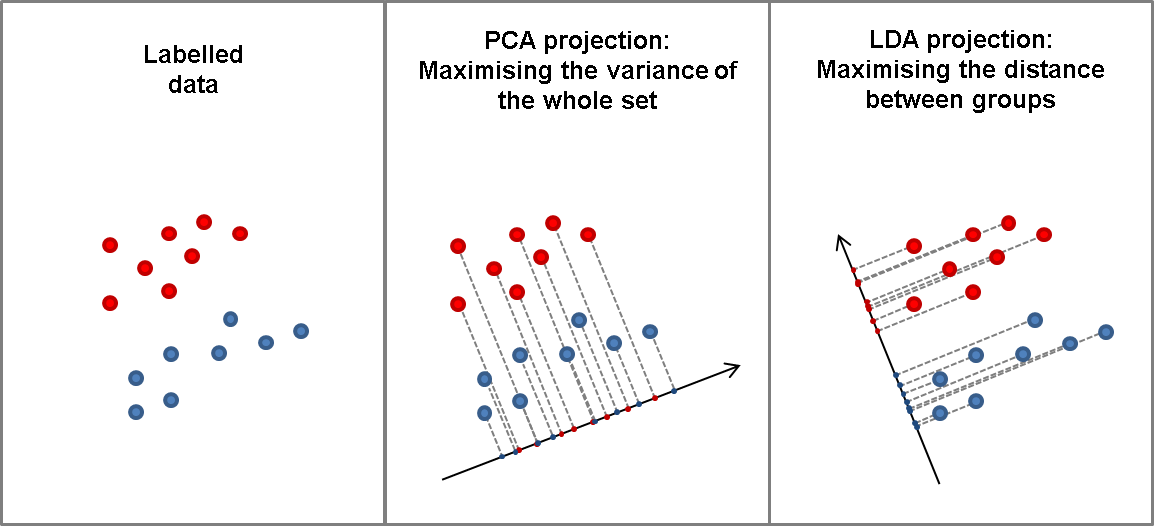
\includegraphics[width=0.7\textwidth]{../resources/methods/lda.png}
    \end{figure}
\end{frame}

\begin{frame}{Canonical Correlation Analysis (CCA)}
    \textbf{Цель:} Найти коррелирующие компоненты в двух наборах данных.

    \textbf{Пример применения:}
    \begin{itemize}
        \item Связь между анкетными данными и биометрией.
        \item Исследование двух источников данных для выявления зависимостей.
    \end{itemize}
\end{frame}

\subsection{Нелинейные методы}

\begin{frame}{Kernel PCA (KPCA)}
    \textbf{Ключевая идея:} \textit{Kernel Trick} для проецирования в нелинейное пространство.

    Пример ядерной функции (гауссовское ядро):
    \begin{equation*}
        k(\mathbf{x}_i, \mathbf{x}_j) = \exp\left(-\frac{\|\mathbf{x}_i - \mathbf{x}_j\|^2}{2\sigma^2}\right)
    \end{equation*}

    \textbf{Пример применения:}
    \begin{itemize}
        \item Обнаружение сложных текстур на изображениях.
        \item Биоинформатика: анализ активности молекул.
    \end{itemize}
\end{frame}


\begin{frame}{Kernel PCA (KPCA)}
    \begin{figure}
        \centering
        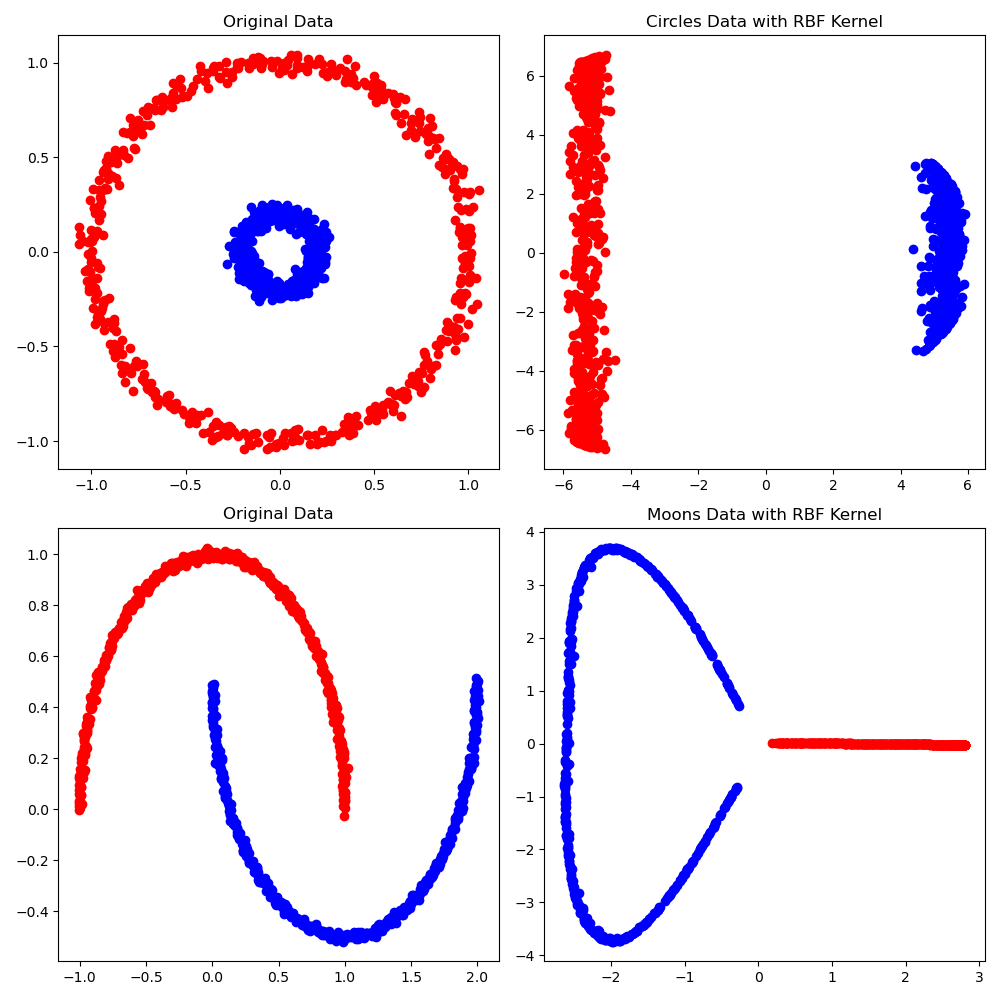
\includegraphics[width=.5\textwidth]{../resources/methods/kpca.png}
    \end{figure}
\end{frame}

\begin{frame}{t-SNE}
    Алгоритм визуализации (!) данных высокой размерности.

    \textbf{Цель:} Локальное сохранение расстояний между точками.

    Основная идея:
    \begin{itemize}
        \item Перевод данных в вероятностное представление.
        \item Минимизация расстояния Кульбака-Лейблера (KL-дивергенция).
    \end{itemize}

    \textbf{Пример применения:}
    \begin{itemize}
        \item Визуализация эмбеддингов слов или изображений.
        \item Кластеризация геномных данных.
    \end{itemize}
\end{frame}

\begin{frame}{t-SNE}
    \begin{figure}
        \centering
        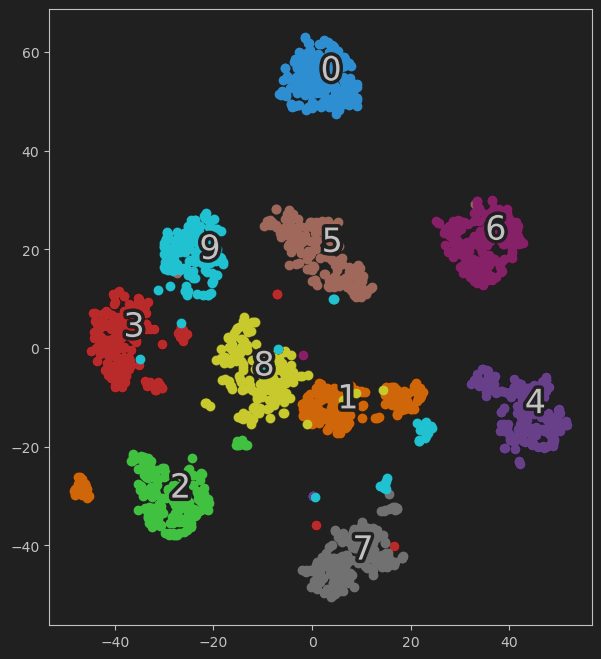
\includegraphics[width=0.6\textwidth]{../resources/methods/tsne.png}
    \end{figure}
\end{frame}

\begin{frame}{UMAP (\textit{Uniform Manifold Approximation and Projection})}
    \textbf{Цель:} Сохранение как локальных, так и глобальных структур данных.

    Основные этапы метода:
    \begin{itemize}
        \item Построение графа соседей данных в исходном пространстве.
        \item Оптимизация аппроксимации графа в пространстве меньшей размерности.
    \end{itemize}

    \textbf{Пример применения:}
    \begin{itemize}
        \item Визуализация паттернов активности мозга.
        \item Анализ биоинформационных данных.
    \end{itemize}
\end{frame}

\begin{frame}{UMAP (\textit{Uniform Manifold Approximation and Projection})}
    \begin{figure}
        \centering
        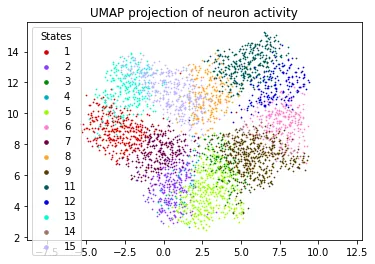
\includegraphics[width=0.7\textwidth]{../resources/methods/umap.png}
    \end{figure}
\end{frame}

\begin{frame}{AutoEncoders (AEs)}
    \textbf{Цель:} Нахождение компактных нелинейных представлений данных.

    Основная структура:
    \begin{itemize}
        \item Кодировщик (encoder): преобразует входные данные в компактное представление.
        \item Декодировщик (decoder): восстанавливает данные из сжатого представления.
    \end{itemize}

    \textbf{Пример применения:}
    \begin{itemize}
        \item Удаление шума с изображений.
        \item Выделение особенностей для классификации.
    \end{itemize}
\end{frame}

\begin{frame}{AutoEncoders (AEs)}
    \begin{figure}
        \centering
        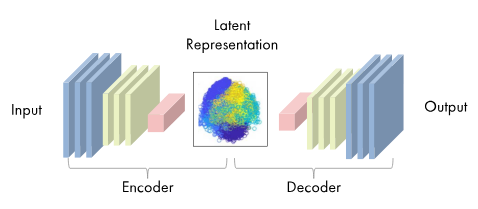
\includegraphics[width=0.85\textwidth]{../resources/methods/autoencoder.png}
    \end{figure}
\end{frame}

\begin{frame}{Variational AutoEncoders (VAEs)}
    \textbf{Расширение автоэнкодеров:} генерация данных на основе латентного пространства.

    Основная идея:
    \begin{itemize}
        \item Представление латентного пространства в виде вероятностного распределения.
    \end{itemize}

    \textbf{Пример применения:}
    \begin{itemize}
        \item Генерация новых молекул с заданными свойствами.
        \item Создание искусственных изображений.
    \end{itemize}
\end{frame}

\begin{frame}{Variational AutoEncoders (VAEs)}
    \begin{figure}
        \centering
        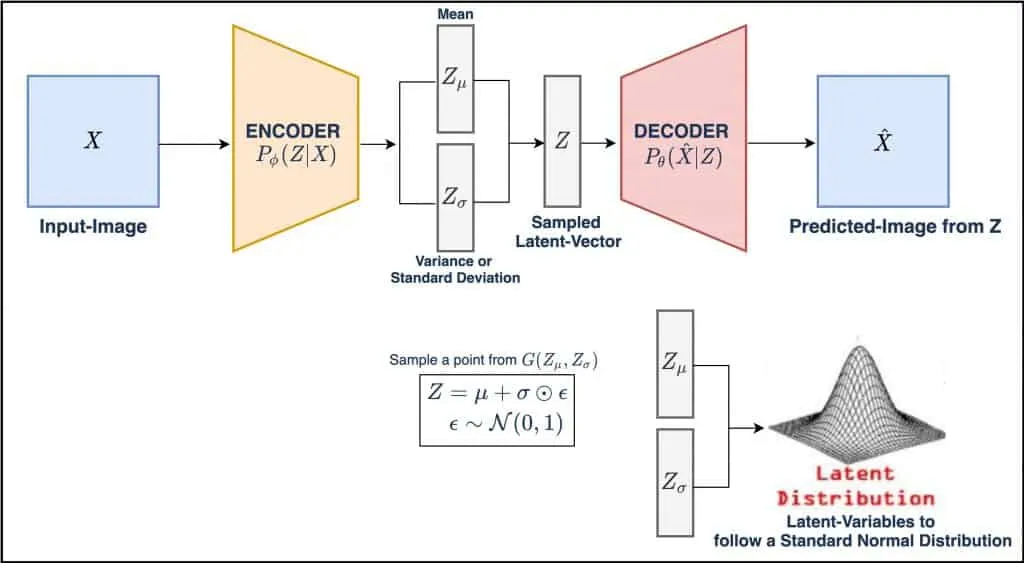
\includegraphics[width=0.9\textwidth]{../resources/methods/vae.png}
    \end{figure}
\end{frame}
